\documentclass[11pt]{article}
\usepackage[utf8]{inputenc}
\usepackage{amsmath,amssymb}
\usepackage{graphicx}
\usepackage{hyperref}
\usepackage{geometry}
\geometry{margin=1in}

% --- TikZ and PGFPlots for waveforms ---
\usepackage{tikz}
\usepackage{pgfplots}
\pgfplotsset{compat=1.18}  % or a suitable version you have

\title{A Hierarchical Framework of Emotion Using EOR and Good/Bad Valued Logic}
\author{Brian Searls}
\date{\today}

\begin{document}

\maketitle

\begin{abstract}
This paper outlines a hierarchical model of emotions based on an Event-Outcome-Response (EOR) framework and Good/Bad valued logic. Emotions are categorized at three levels (L0--L2). At the foundation (L0) are fundamental positive (Good) and negative (Bad) affective signals. Building on these, early discrete emotions (Interest, Disgust) appear at L1. Finally, more complex emotions (Fear, Anger, Sadness, Surprise) emerge at L2 as combinations of lower-level states or continued interactions of Good and Bad signals. The core connections among all nodes are summarized in a single adjacency matrix. To capture temporal dynamics, the Good and Bad signals are represented as time-varying functions \(G(t)\) and \(B(t)\). Waveform examples for Surprise and Fear demonstrate how these signals can evolve. Future work will consider extending this framework to higher-level emotions (L3+).
\end{abstract}

\tableofcontents

\section{Introduction}
Emotions are central to cognition, communication, and behavior. Numerous psychological and computational models have explored their structure, function, and development. In the framework described here, an Event-Outcome-Response (EOR) process is combined with a Good/Bad valued logic to form the basis of a hierarchical theory of emotional emergence. The approach posits that at the lowest level (L0), all affective processes can be reduced to fundamental signals of Good (positive valence) and Bad (negative valence). These signals interact in increasingly complex ways at higher levels (L1 and L2) to yield a variety of emotions observed in humans.

Sections \ref{sec:hierarchy} and \ref{sec:matrix} introduce the three-level structure (L0--L2) and summarize their connections via a single adjacency matrix. Section \ref{sec:dynamics} describes how Good and Bad signals \((G(t), B(t))\) might evolve over time in response to events. Section \ref{sec:waveform-examples} provides waveform examples for Surprise and Fear. Finally, Section \ref{sec:conclusion} offers a brief outlook on future extensions of this model.

\section{Three Levels of Emotional Emergence}
\label{sec:hierarchy}
We propose three levels, reflecting a progression from basic affective signals (L0) to discrete primary emotions (L1) to more complex secondary emotions (L2).

\subsection{L0: Fundamental Good/Bad States}
\begin{itemize}
    \item \textbf{Good (positive valence)}: A fundamental feeling of pleasure, comfort, or satisfaction.  
    \item \textbf{Bad (negative valence)}: A fundamental feeling of discomfort, pain, or distress.
\end{itemize}

\subsection{L1: Early Emotions (Interest, Disgust)}
\begin{itemize}
    \item \textbf{Interest}: A positive, exploratory state triggered by novelty or an anticipated opportunity (primarily Good with a hint of bad).  
    \item \textbf{Disgust}: An aversive response to something judged unpleasant, harmful, or offensive (primarily Bad with a hint of good).
\end{itemize}

\subsection{L2: Complex Emotions (Fear, Anger, Sadness, Surprise)}
\begin{itemize}
    \item \textbf{Fear}: Triggered by a perceived threat, often combining a strong Bad signal with alarm or attention.  
    \item \textbf{Anger}: Frequently arises from blocked goals or perceived injustice, reflecting both Good (a desired outcome) and Bad (the obstacle or violation).  
    \item \textbf{Sadness}: A sustained negative state tied to the loss of something Good or an enduring adversity.  
    \item \textbf{Surprise}: A brief, intense reaction to unexpected events, potentially involving both a startle (negative) and a spark of interest (positive).
\end{itemize}

\section{Adjacency Matrix of Connections}
\label{sec:matrix}
Below is a single adjacency matrix summarizing how each node (L0--L2) influences every other node. The diagonal is marked with “--” to indicate no self-connection, and we replace explicit “None” with a dash “-” for brevity. Other descriptors (e.g., “Strong,” “Partial,” “Brief,” “Sustained”) indicate the qualitative nature of each influence.

\begin{table}[htbp]
\centering
\renewcommand{\arraystretch}{1.15}
\resizebox{\textwidth}{!}{%
\begin{tabular}{l|cccccccc}
\hline
 & \textbf{Good(L0)} & \textbf{Bad(L0)} & \textbf{Interest(L1)} & \textbf{Disgust(L1)} & \textbf{Fear(L2)} & \textbf{Anger(L2)} & \textbf{Sadness(L2)} & \textbf{Surprise(L2)} \\
\hline
\textbf{Good(L0)}      & -- & - & Strong & Weak & - & Partial & Sustained & Partial \\
\textbf{Bad(L0)}       & - & -- & Weak & Strong & Strong & Partial & Strong & Partial \\
\textbf{Interest(L1)}  & - & - & -- & - & Strong & Partial & - & Brief \\
\textbf{Disgust(L1)}   & - & - & - & -- & Partial & Strong & - & Brief \\
\textbf{Fear(L2)}      & - & - & - & - & -- & - & - & - \\
\textbf{Anger(L2)}     & - & - & - & - & - & -- & - & - \\
\textbf{Sadness(L2)}   & - & - & - & - & - & - & -- & - \\
\textbf{Surprise(L2)}  & - & - & - & - & - & - & - & -- \\
\hline
\end{tabular}
}
\caption{Adjacency matrix for L0--L2 nodes. Each cell indicates the qualitative nature of influence. The diagonal is ``--'' to denote no self-connections.}
\label{tab:adjacency-matrix}
\end{table}

\section{Temporal Dynamics of Good/Bad Signals}
\label{sec:dynamics}
Beyond these structural connections, each emotion can be viewed as a pattern in two time-dependent signals:
\[
G(t) \quad\text{(Good component)}, 
\quad 
B(t) \quad\text{(Bad component)},
\]
where events in the EOR framework may raise or lower one or both for a period. Different emotions correspond to distinct profiles of \(G(t)\) and \(B(t)\).

\subsection{Illustrative Formalism}
A simple model uses exponential decays for each event:
\[
G(t) \;=\; \sum_{i} \Delta G_i \, e^{-\alpha (t - t_i)}\, H(t - t_i), 
\quad
B(t) \;=\; \sum_{j} \Delta B_j \, e^{-\beta (t - s_j)}\, H(t - s_j),
\]
where \(\Delta G_i\) and \(\Delta B_j\) are amplitudes, \(t_i\) and \(s_j\) are event times, and \(\alpha,\beta\) set decay rates. The function \(H\) is a step that ensures no contribution occurs before the event. Different emotional states then emerge depending on how high or low \(G(t)\) and \(B(t)\) become over time.

\section{Waveform Examples: Surprise and Fear}
\label{sec:waveform-examples}
Below we present two examples illustrating how \(G(t)\) and \(B(t)\) might evolve under different scenarios.

\subsection{Surprise}
Surprise often involves a simultaneous positive (interest-like) spike and a negative (startle) spike. In Figure~\ref{fig:surprise-waveform}, an event at \(t=1\) triggers both.

\begin{figure}[htbp]
\centering
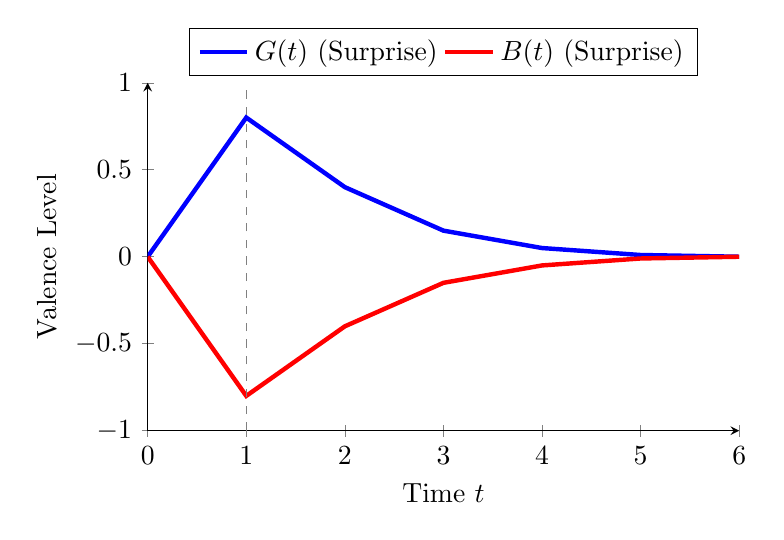
\begin{tikzpicture}
\begin{axis}[
    width=0.75\textwidth,
    height=6cm,
    xmin=0, xmax=6,
    ymin=-1, ymax=1,
    axis lines=left,
    xlabel={Time $t$},
    ylabel={Valence Level},
    ytick={-1, -0.5, 0, 0.5, 1},
    legend style={at={(0.5,1.02)},anchor=south,legend columns=2}
]
% G(t) for Surprise
\addplot[blue, ultra thick] coordinates {
    (0, 0)
    (1, 0.8)
    (2, 0.4)
    (3, 0.15)
    (4, 0.05)
    (5, 0.01)
    (6, 0)
};
\addlegendentry{$G(t)$ (Surprise)}

% B(t) for Surprise (negative axis)
\addplot[red, ultra thick] coordinates {
    (0, 0)
    (1, -0.8)
    (2, -0.4)
    (3, -0.15)
    (4, -0.05)
    (5, -0.01)
    (6, 0)
};
\addlegendentry{$B(t)$ (Surprise)}

% Dashed event line
\draw[dashed,gray] (axis cs:1,-1) -- (axis cs:1,1)
    node[above,pos=1,black]{Event at $t=1$};

\end{axis}
\end{tikzpicture}
\caption{Hypothetical Surprise response with spikes in both $G(t)$ and $B(t)$. Both decay relatively quickly afterward.}
\label{fig:surprise-waveform}
\end{figure}

\subsection{Fear}
A Fear response features a strong rise in negative valence with little or no positive component. Figure~\ref{fig:fear-waveform} shows an event at \(t=2\) that drives \(B(t)\) upward (plotted below the axis) while \(G(t)\) remains near zero.

\begin{figure}[htbp]
\centering
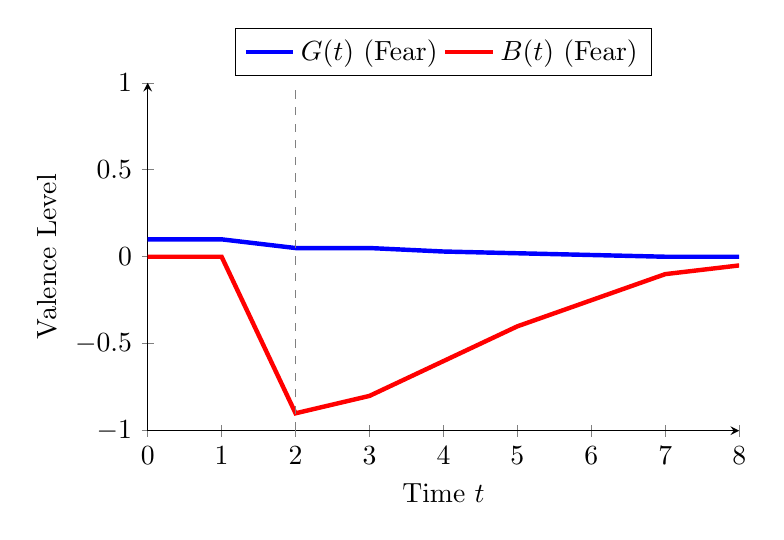
\begin{tikzpicture}
\begin{axis}[
    width=0.75\textwidth,
    height=6cm,
    xmin=0, xmax=8,
    ymin=-1, ymax=1,
    axis lines=left,
    xlabel={Time $t$},
    ylabel={Valence Level},
    ytick={-1, -0.5, 0, 0.5, 1},
    legend style={at={(0.5,1.02)},anchor=south,legend columns=2}
]
% G(t) for Fear
\addplot[blue, ultra thick] coordinates {
    (0, 0.1)
    (1, 0.1)
    (2, 0.05)
    (3, 0.05)
    (4, 0.03)
    (5, 0.02)
    (6, 0.01)
    (7, 0)
    (8, 0)
};
\addlegendentry{$G(t)$ (Fear)}

% B(t) for Fear
\addplot[red, ultra thick] coordinates {
    (0, 0)
    (1, 0)
    (2, -0.9)
    (3, -0.8)
    (4, -0.6)
    (5, -0.4)
    (6, -0.25)
    (7, -0.1)
    (8, -0.05)
};
\addlegendentry{$B(t)$ (Fear)}

% Dashed event line
\draw[dashed,gray] (axis cs:2,-1) -- (axis cs:2,1)
    node[above,pos=1,black]{Event at $t=2$};

\end{axis}
\end{tikzpicture}
\caption{Hypothetical Fear response. $B(t)$ spikes at $t=2$ while $G(t)$ remains near zero. The negative affect can linger if the threat is perceived to persist.}
\label{fig:fear-waveform}
\end{figure}

\section{Conclusion and Outlook}
\label{sec:conclusion}
This paper presented a hierarchical model of emotions based on an Event-Outcome-Response process and Good/Bad valued logic. Three main levels were described: foundational valences (L0), early discrete emotions (L1), and more complex secondary emotions (L2). An adjacency matrix summarized node-to-node influences, and time-dependent signals \(G(t)\) and \(B(t)\) illustrated how an event could spark different emotional profiles over time.

Future research may address L3 and beyond, potentially including self-conscious emotions (e.g., shame, guilt, pride) which build on these foundations with richer cognitive appraisals. By preserving the Good/Bad logic, the model can extend to more advanced emotional processes without losing its core simplicity. Potential applications include developmental psychology, affective computing, and AI systems designed to interpret or simulate emotional states in a structured, hierarchical manner.

\end{document}
